%%%%%%%%%%%%%%%%%%%%%%%%%%%%%%%%%%%%%%%%%
% Stylish Article
% LaTeX Template
% Version 2.1 (1/10/15)
%
% This template has been downloaded from:
% http://www.LaTeXTemplates.com
%
% Original author:
% Mathias Legrand (legrand.mathias@gmail.com) 
% With extensive modifications by:
% Vel (vel@latextemplates.com)
% Final ACS by:
% Juan Barbosa
% License:
% CC BY-NC-SA 3.0 (http://creativecommons.org/licenses/by-nc-sa/3.0/)
%
%%%%%%%%%%%%%%%%%%%%%%%%%%%%%%%%%%%%%%%%%
\documentclass[fleqn,10pt]{SelfArx}
%\usepackage[superscript]{cite}
\usepackage{wrapfig}
\usepackage{multirow}
%----------------------------------------------------------------------------------------
%	ARTICLE INFORMATION
%----------------------------------------------------------------------------------------

\JournalInfo{Laboratorio de Bioquímica, No. 1, 05/02/2019} % Journal information
\Archive{ }

\PaperTitle{Fraccionamiento de tejidos e identificación de sus principales constituyentes} %
%\Keywords{Keyword1 --- Keyword2 --- Keyword3} % Keywords - if you don't want any simply remove all the text between the curly brackets
%\newcommand{\keywordname}{Keywords} % Defines the keywords heading name

%----------------------------------------------------------------------------------------
%	ABSTRACT
%----------------------------------------------------------------------------------------

\Abstract{The extraction and analysis of biological components such as carbohydrates, lipids and proteins is of vital importance for medicine and biochemistry. Because of this importance, qualitative tests have been developed, such as Lugol, Molish, Saponification, Benedict, Biuret and Ninhydrin, being these the ones studied on this document using animal tissues, to identify the presence of carbohydrates, lipids and proteins in the different samples. In order to isolate these compounds we carried out a tissue fractionation using centrifuge related procedures. Results show the presence of carbohydrates, lipids and proteins in all the studied samples. Nevertheless there are contradicting results associated to specific tests and samples, that made impossible to accurately relate the results from the different tissues.
}

%----------------------------------------------------------------------------------------

\begin{document}

\flushbottom % Makes all text pages the same height

\maketitle % Print the title and abstract box
%\tableofcontents % Print the contents section

\thispagestyle{empty} % Removes page numbering from the first page



%----------------------------------------------------------------------------------------
%	ARTICLE CONTENTS
%----------------------------------------------------------------------------------------

\section*{Introducci\'on} % The \section*{} command stops section numbering
%------------------------------------------------
	La extracción y/o análisis de componentes biológicos cómo lo son los carbohidratos, los lípidos y las proteínas es de vital importancia para la medicina y la bioquímica, ya que permite detectar ciertas enfermedades o caracterizar la composición de diferentes órganos para ver estos cómo pueden ser afectados por diferentes agentes externos. Muchas de las técnicas de análisis de estos componentes son de carácter cualitativo, y dependen de cambios de color o de apariencia para comprobar la presencia de estos compuestos en diversas muestras orgánicas. 
	
	La técnica más antigua relevante a este trabajo es la saponificación. La saponificación es un método usado desde la antigüedad para fabricar jabón, en el cual se convierten ácidos grasos en sales metálicas de estos mismos ácidos \cite{preston1925modern}, los cuales son usados como jabón debido a que estas sales tienen tanto una parte hidrofóbica como una parte hidrofílica \cite{preston1925modern}. Al formarse un producto fácilmente observable al ser agitado en solución acuosa, el proceso de saponificación es útil para el análisis cualitativo de lípidos \cite{souza2017microwave}. Este proceso también puede ser utilizado para la separación de metales de tierras raras \cite{dong2016sustainable}.
	Cronológicamente sigue la prueba con el reactivo de Lugol, desarrollado en 1829 por el químico francés Jean Lugol \cite{sneader2005drug} el cual tiene diversos usos médicos cómo la detección de cáncer de cerviz \cite{novak1937pseudomalignant}, la detección de displasia esofágica \cite{li2018lugol} y la disminución de sangrado intraoperatorio \cite{yilmaz2016effect}. Este reactivo es utilizado tanto para estas pruebas médicas como indicador de carbohidratos debido a que el yodo presente en el reactivo se añade a la estructura de polisacáridos, polisacáridos cuya concentración disminuye en tejido enfermo como el tejido del cáncer de cerviz.
	
	\newpage
	La siguiente es la prueba de Biuret, descrita por el científico polaco Gregor van Piotrowski en 1857 \cite{von1857neue} la cual es usada para la determinación de proteínas en muestras biológicas al formarse complejos de coordinación morados en presencia de péptidos \cite{rose1833ueber}. La prueba de Biuret es utilizada para cuantificar la proteína en suero biológico con incertidumbres aceptables \cite{zheng2017measurement} y para la detección de proteínas en acero quirúrgico con tal de prevenir la transmisión de priones iatrogénicos \cite{lipscomb2006sensitivity}.
	
	Sigue la prueba Liebermann-Burchard, desarrollada entre 1885 y 1889 \cite{xiong2007liebermann} utilizada para la detección de lípidos, principalmente colesterol, en muestras orgánicas \cite{barreto2005lipid}. en la prueba el ácido sulfúrico reacciona con el grupo hidroxilo del colesterol para formar colestapolenos conjugados que dan la coloración verde esperada \cite{xiong2007liebermann, burke1974mechanisms}. En la actualidad también se utiliza la prueba de Zak, la cual tiene un mecanismo de oxidación similar al de la prueba Liebermann-Burchard pero utiliza \ce{Fe^{3+}} para formar colestapolenos de color rojo \cite{burke1974mechanisms}.
	
	Entre 1908 y 1910 se desarrollaron 3 diferentes métodos de análisis de diversos componentes biológicos, el primero de estos fue la prueba de Benedict, desarrollada en 1908\cite{benedict1909reagent} por el químico estadounidense Stanley Benedict. Esta prueba es utilizada para identificar azucares reductores simples debido a que estas azucares pueden reducir el Cu(II) presente en el reactivo de benedict a Cu(I) \cite{daniels1960fehling}, causando un cambio de coloración de azul a rojo intenso. 

	\begin{figure*}[h]
		\centering
		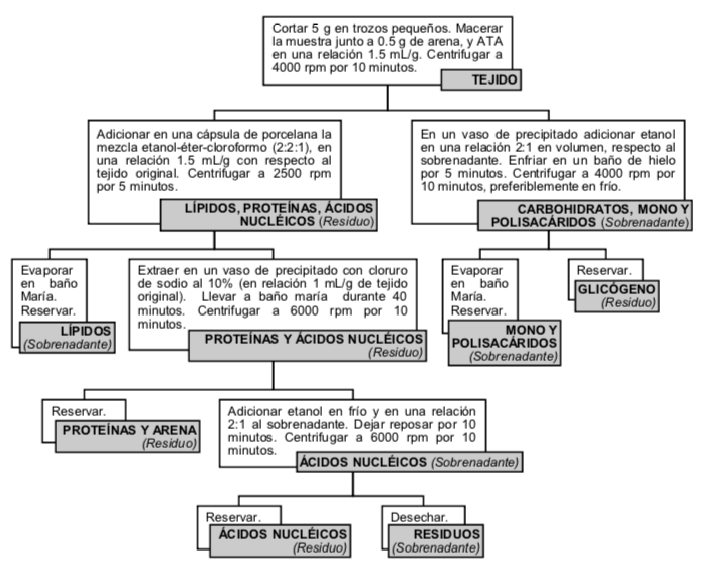
\includegraphics[width = 0.7\linewidth]{fraccionamiento.png}
		\caption{Procedimiento realizado para el fraccionamiento del tejido.}
		\label{fig: fraccionamiento}
	\end{figure*}

	El segundo de estos métodos desarrollados a principios del siglo XX fue la prueba de Molisch, cuyo principio básico fue investigado por Van Ekestein y Blanksma en 1909 \cite{van1910omega}. La prueba requiere de la formación de furfural o 5-hidroximetilfurfural a partir de pentosas y hexosas respectivamente, las cuales se unen a moléculas de $\alpha$-naftol presentes en el reactivo para formar un compuesto con coloración morada \cite{devor1950carbohydrate}. 
	
	\newpage
	
	El último de estos métodos de análisis de componentes biológicos de muestras biológicas es la prueba con Ninhidrina, cuyo reactivo principal fue descubierto por el químico alemán Siegfried Ruhemann en 1910 \cite{ruhemann1910cxxxii, ruhemann1910ccxii}. La ninhidrina reacciona con el grupo amino de los aminoácidos para formar un producto de coloración morada, el cual es conocido como morado de Ruhemann. Puede ser usado tanto cualitativamente como cuantitativamente, siendo la ninhidrina utilizada para detectar glifosatos con espectroscopía Raman \cite{xu2018indirect}, para realizar secuenciación de péptidos \cite{friedman2004applications} y para determinar el sexo de una persona a partir de residuos encontrados en huellas dactilares \cite{brunelle2016new}. 
	
	Todos estos métodos varían en términos de especificidad y precisión, pero todos son útiles a la hora de determinar la presencia de los diversos compuestos que se desean encontrar en diferentes tejidos humanos y animales, por lo que el objetivo del presente es demostrar la presencia de diversas clases de carbohidratos, lípidos y proteínas en muestras biológicas y compararlas en función de su composición. 
	
\section{Secci\'on experimental}
	\subsection{Preparación de las soluciones}
		Se prepararon las soluciones como se describe a continuación:
		\begin{enumerate}
			\item \textbf{Ácido clorhídrico al 10 \% v/v:} Se tomaron 2.7 mL de ácido clorhídrico concentrado (37 \%) y se llevó a 10 mL con agua.
			\item \textbf{Hidróxido de sodio al 15 \% p/v:} Se tomaron 1.5 g de hidróxido de sodio y se llevó a 10 mL con agua.
			\item \textbf{Reactivo de Benedict:} Se pesaron 0.18 g de sulfato de cobre (II) pentahidratado, 0.5 g de carbonato de sodio y 0.85 g de citrato de sodio, y se llevó a 10 mL de agua. Agite bien.
			\item \textbf{Reactivo de Biuret:} Se disolvieron 15 mg de sulfato de cobre (II) pentahidratado y 60 mg de tartrato de sodio y potasio tetrahidratado, en 5 mL de agua. Se añadió luego 2 mL de la solución de hidróxido de sodio al 15 \% preparada anteriormente. Posteriormente se adicionó 10 mg de yoduro de potasio. Finalmente se llevó a 10 mL con agua. El reactivo fue almacenado en una botella ámbar pequeña.
			\item \textbf{Reactivo de Molisch:} Se disolvieron 0.1 g de $\alpha$-Naftol en 1 mL de etanol absoluto.
			\item \textbf{Lugol:} Se disolvieron 18 mg de yodo sólido en polvo y 32 mg de yoduro de potasio en polvo en 5 mL de agua. Se agitó vigorosamente hasta la disolución completa de los reactivos. Se cubrió el beaker con papel aluminio.
			\item \textbf{Nihidrina al 0.2 \%:} Se disolvieron 10 mg de ninhidrina en 5 mL de etanol absoluto.
			\item \textbf{Cloruro de sodio al 10 \%:} Se tomó 1 g de cloruro de sodio y se llevó a 10 mL con agua.
			\item \textbf{Éter-Etanol-Cloroformo (2:2:1):} Se Mezclaron 4 mL de éter etílico, 4 mL de etanol absoluto y 2
			mL de cloroformo.
			\item \textbf{Ácido tricloroacético al 10 \%:} Se pesó 1 g de ácido tricloroacético y se llevó a 10 mL con agua.
		\end{enumerate}
	\subsection{Fraccionamiento del tejido}
		Se realizó el fraccionamiento de los órganos por grupos independientes siguiendo la \autoref{fig: fraccionamiento}. Los órganos estudiados de manera independiente por los grupos de laboratorio, incluyen: hígado de res, cerebro de res, hígado de pollo y corazón de pollo.
		
	\subsection{Pruebas de identificación}
		Con las muestras obtenidas se realizaron las siguientes pruebas de identificación:
		\subsubsection{Análisis de carbohidratos}
			La muestra se dividió en cuatro fracciones:
			\begin{enumerate}
				\item A la primera se le agregaron 3 gotas de Lugol y se observó el cambio de coloración de la muestra.
				\item A la segunda se le adicionó 1 mL de la solución de ácido clorhídrico al 10 \% y se colocó al baño María por 25 minutos. Se dejó enfriar y se agregaron 3 gotas de Lugol, se observó el cambio de coloración de la muestra.
				\item A la tercera se le adicionó 1 mL de agua destilada y 3 gotas del reactivo de Molisch. Luego se agregó 1 mL de ácido sulfúrico concentrado sin mezclar las dos fases formadas. Se observó la coloración de la muestra.
				\item Se ubicó la cuarta fracción al baño María por 2 minutos, luego se adicionaron 2 mL del reactivo de Benedict. Se observó la coloración en ese momento y 10 minutos después de dejarse en calentamiento. 
			\end{enumerate}
		\subsubsection{Análisis de lípidos}
			La muestra se dividió en 2 fracciones:
			\begin{enumerate}
				\item A la primera se le adicionó 3 mL de cloroformo y se mezcló. Luego se adicionó 1 mL de anhídrido acético. Tras esto se agregaron 3 gotas de ácido sulfúrico. Se observó la coloración de la interfase tras 1 minuto, y después de 15 minutos.
				\item A la segunda se le agregaron 3 mL de hidróxido de sodio al 15 \%. Luego se ubicó al baño maría durante 20 minutos. Finalmente se adicionaron 3 mL de agua destilada y se agitó fuertemente. 
			\end{enumerate}
		
		\subsubsection{Análisis de proteínas}
			La muestra se dividió en 2 fracciones:
			\begin{enumerate}
				\item A la primera se le adicionó 1 mL de agua destilada y se suspendió la muestra. Se agregó 1 mL del reactivo de Biuret y se observó el cambio de coloración.
				\item A la segunda se le agregó 1 mL de la solución de ninhidrina y se calentó al baño María por 10 minutos.
			\end{enumerate}

	\begin{table*}[h!]
	\small
	\caption{Resultados obtenidos para los distintos tejidos con las pruebas espec\'ificas a carbohidratos.}
	\label{tb: carbohidratos}
	\begin{tabular}{p{1.5cm}|p{3.5cm}p{3.5cm}p{3.5cm}p{3.5cm}}
		\hline
		\textbf{Tejido} & \textbf{1. Prueba Lugol} & \textbf{2. Prueba ácido + lugol} & \textbf{3. Reacción de Molish} & \textbf{4. Reacción de Benedict}
		\\
		\hline
		\textbf{H\'igado de pollo} & La solución inicial de coloración amarilla no presentó ningún cambio & Tampoco se evidenció algún cambio en la solución & Se observó la formación de un anillo color violeta & La solución inicial presentaba una coloración azul. Se observó la formación de un precipitado verde
		\\
		\hline
		\textbf{H\'igado de pollo} & La coloración amarilla de la solución inicial se mantuvo, la prueba no dió & Tampoco dió & Se observó la formación del anillo morado esperado & No se observó el cambio de coloración esperado o la formación de un precipitado verde, la prueba no dió
		\\
		\hline
		
		\textbf{H\'igado de res} & La solución no cambio su coloración amarilla inicial, pero en la parte inferior del tubo se tornó amarillo mas intenso & La solución tampoco cambio su coloración amarilla inicial, y la parte inferior del tubo tambi\'en se tornó amarillo mas intenso	& Se observó la formaci\'on de un anillo color morado en la parte inferior & Primero se observó una coloraci\'on azul tenue en la parte superior y azul fuerte en la parte inferior del tubo. Despu\'es de calentamiento tomo una coloraci\'on verde tenue en la parte superior y fuerte en la inferior.
		\\
		\hline
		
		\textbf{H\'igado de res} & La solución tomó un color amarillo pálido correspondiente a la adición del reactivo, no se observa ningún cambio & No se observa un cambio aparente con respecto a su color inicial (amarillo pálido) & Se observa la formación de un anillo de color morado entre las fases presentes & La muestra es incolora, al adicionar el reactivo toma un color azul y luego de 10 minutos de calentamiento vira al verde
		\\
		\hline
		
		\textbf{Coraz\'on de pollo} & La solución arrojó una coloración cafe rojizo & Color amarillo sin algun cambio representativo & Se formaron dos fases y un anillo violeta & No hubo precipitado, ni cambio de color
		\\
		\hline
		
		\textbf{Coraz\'on de pollo} & La solucion se mantuvo amarilla, no hubo cambio en la coloracion & No se vio cambio de color	& Se formaron dos fases y en la interfase se vio un anillo morado & No reacciono. Sin cambio de color y sin precipitado rojo.
		\\
		\hline
		
		\textbf{Cerebro de res} & No dio & Inicialmente se presentó una coloración amarilla en el fondo, la cual fue desapareciendo con el tiempo. & Se observó la formación de un anillo color amarillo tenue. & La prueba arrojó coloraci\'on azul
		\\
		\hline
		\textbf{Cerebro de res} & No se observó un cambio de color & No se observó un cambio de color & Se observó la formación de dos fases. La fase que estaba en la parte más superficial se tornó de un color rojo. Tras la adición de una mayor cantidad de ácido sulfúrico se observó lentamente la formación del anillo color negro en la interfase & No se observó un cambio de color
		\\
		\hline
	\end{tabular}
\end{table*}

	\begin{table*}[h!]
	\small
	\caption{Resultados obtenidos para los distintos tejidos con las pruebas espec\'ificas a l\'ipidos.}
	\label{tb: lipidos}
	\begin{tabular}{p{2.5cm}|p{7cm}p{7cm}}
		\hline
		\textbf{Tejido} & \textbf{1. Prueba Salkowsky} & \textbf{2. Prueba NaOH}
		\\
		\hline
		\textbf{H\'igado de pollo} & Se observó la formación de dos capas, la superior de color verde claro y la inferior rojiza & Se observó la formación de dos capas, la superior con textura espesa. Tras calentar se tornó rojiza. 
		\\
		\hline
		\textbf{H\'igado de pollo} & No se observó la formación de las dos fases esperadas, la prueba no dió & Se observó un cambio de coloración a un color verde oscuro, el cual cambió a café al calentarse, la prueba dió.
		\\
		\hline
		
		\textbf{H\'igado de res} & Se observo la formaci\'on de dos capas, la superior verde muy tenue casi blanco, la inferior cafe claro y una pequeña capa caf\'e oscura entre las dos anteriores & Al inicio se ten\'ian tres capas de coloraci\'on vinotinto, rojiza y amarilla muy tenue, pero despu\'es de calentamiento tomo una coloraci\'on caf\'e/verde
		\\
		\hline
		
		\textbf{H\'igado de res} & La muestra presenta una coloración rojiza luego de la adición del ácido, cuando se calienta se torna de color café & Se observa en un inicio una solución de color rojo intenso, a medida que se calentó tomó un color verde
		\\
		\hline
		
		\textbf{Coraz\'on de pollo} & Se observó la formaci\'on de dos capas: de color caf\'e claro y blanco & Se observó una solución poco turbia y de color caf\'e verdoso
		\\
		\hline
		
		\textbf{Coraz\'on de pollo} & Al minuto se vio la formaci\'on de dos fases separadas por un anillo naranja. Despu\'es de 15 minutos el anillo se hab\'ia tornado café & La soluci\'on se volvi\'o verde, con el calentamiento se tornó caf\'e y finalmente volvi\'o a tomar coloraci\'on verdosa
		\\
		\hline
		
		\textbf{Cerebro de res} & No se observó precipitado & La muestra cambió a verde, al calentar se tornó café y por último volvió a verde
		\\
		\hline
		\textbf{Cerebro de res} & Tras la adición de cloroformo se formaron dos fases y la muestra se tornó color pastel. Después de adicionar anhídrido acético se obtuvo una fase. Finalmente, al agregar ácido sulfúrico se observa la formación de una tercera fase con un anillo color negro en la interfase & Al agregar NaOH la muestra cambió a un color verde. Conforme el tiempo pasó, se formaron dos fases. La superior con un color verde oscuro y la inferior con un color verde claro. Con calentamiento la fase superior cambió a color rojo mientras que la inferior cambiaba lentamente a un color amarillo. Finalmente, tras la adición de agua y agitación se formaron dos fases: una verde uniforme y otra blanca de apariencia espumosa.
		\\
		\hline
	\end{tabular}
\end{table*}

\section{Resultados y Discusi\'on}
	Según los resultados obtenidos para el análisis de carbohidratos, los cuales se muestran en la \autoref{tb: carbohidratos}, se pudo descartar la presencia de polisacáridos en la muestra, puesto que no se observó el cambio de coloración en la muestra a causa de la adición del Lugol. Lo anterior debido a que esta última es producto de la introducción del yodo, presente en el reactivo, en la estructura molecular de los polisacáridos, por lo que no es posible identificar monosacáridos por medio de esta prueba. Adicionalmente, los resultados obtenidos con la segunda muestra, luego del tratamiento con ácido clorhídrico, permiten confirmar la ausencia de polisacáridos en la misma, puesto que los enlaces glucosídicos se hidrolizan con facilidad por acción de ácidos como el ácido clorhídrico, al se un ácido prótico que promueve la hídrolisis de la unión covalente del enlace glucosídico de los carbohidratos presentes en la muestra, por lo que la ausencia de coloración es congruente con los resultados obtenidos anteriormente. 
	
	Sin embargo, como se mencionó anteriormente, la prueba con Lugol sólo permite la identificación o presencia de polisacáridos en una muestra, por lo que se llevó a cabo una tercera prueba por medio de la adición del reactivo de Molish. Se observó la formación de un anillo de color morado en la interfase de las dos fases distinguibles, puesto que en general los azúcares se deshidratan en presencia del ácido sulfúrico concentrado, promoviendo de esta manera la formación de compuestos furfúricos que reaccionan con el alfa naftol presente en el reactivo de Molish, causando la coloración observada; de manera que se puede confirmar la presencia de carbohidratos en la muestra. Adicionalmente, la falta de coloración del medio en la cuarta muestra nos permite confirmar la ausencia de azúcares reductores (esto sería teniendo en cuenta que reportaron mal los resultados y en realidad había una tenue coloración azul). Sin embargo, fue posible observar que los resultados diferían en otros grupos durante la experimentación, para los cuales el cambio de color variaba entre azul y verde, lo que se puede explicar porque los grupos reductores aldehídos de algunos azúcares reducen los iones de Cobre a Oxido Cuproso bajo la acción del calor y en medio alcalino, produciendo un cambio en el color del medio desde azul, pasando por verde, naranja y rojo, lo cual depende directamente de la concentración de sustancias reductoras en la muestra y para lo cual se interpreta el azul como negativo, el verde como la presencia de trazas y el amarillo, naranja y rojo como positivo. Cabe resaltar que existe una relación positiva entre los resultados de cada grupo, a pesar de diferir entre sí, por lo que se puede confirmar la ausencia de azúcares reductores en la muestra.
	
	\pagebreak
	
	Por otro lado, en cuanto a las pruebas realizadas para lípidos, las cuales se observan en la \autoref{tb: lipidos}, fue posible observar una congruencia general en los resultados obtenidos por todos los grupos. En el caso de la prueba de Salkowsky el anhídrido acético puede reaccionar con el colesterol y otros esteroles en presencia de ácidos fuertes, formando de esta manera un complejo verde-azul al reaccionar con el grupo hidroxilo del compuesto presente en la muestra, por otro lado, es posible determinar la presencia de \'acidos grasos en una muestra por medio de la adición de hidróxido de sodio para dar lugar a la saponificaci\'on de los mismos, lo cual da lugar a la formaci\'on de miscelas, las cuales dependiendo de su concentraci\'on pueden observarse como otra fase, con caracter\'isticas de viscosidad distintas a la fase acuosa, como reporta un grupo con h\'igado de pollo.
	
	\begin{table}[h!]
	\small
	\caption{Resultados obtenidos para los distintos tejidos con las pruebas espec\'ificas a prote\'inas.}
	\label{tb: proteinas}
	\begin{tabular}{p{1.5cm}|p{2.6cm}p{3.5cm}}
		\hline
		\textbf{Tejido} & \textbf{1. Prueba de Biuret} & \textbf{2. Prueba de Ninhidrina}
		\\
		\hline
		\textbf{H\'igado de pollo} & La solución se tornó color violeta & La solución se tornó color violeta
		\\
		\hline
		\textbf{H\'igado de pollo} & La solución se tornó color violeta & No hubo cambio de color
		\\
		\hline
		
		\textbf{H\'igado de res} & La solución se tornó color violeta & La solución se tornó color violeta
		\\
		\hline
		
		\textbf{H\'igado de res} & La solución se tornó color violeta & No hubo cambio de color
		\\
		\hline
		
		\textbf{Coraz\'on de pollo} & La solución se tornó color violeta & No hubo cambio de color
		\\
		\hline
		
		\textbf{Coraz\'on de pollo} & La solución se tornó color violeta & No hubo cambio de color
		\\
		\hline
		
		\textbf{Cerebro de res} & La solución se tornó color violeta & La solución se tornó color violeta
		\\
		\hline
		\textbf{Cerebro de res} & La solución se tornó color violeta & Inicialmente se observó la formación de una fase color anaranjado. Finalmente, tras un tiempo se observó la formación de una fase color morado con mayor extensión a la naranja
		\\
		\hline
	\end{tabular}
\end{table}

	
	\pagebreak
	Finalmente, para las prote\'inas se obtuvieron los resultados que se muestran en la \autoref{tb: proteinas}. En particular, se puede observar que todas las pruebas de Biuret dieron positivas, esto se debe a que el cobre (II) en soluci\'on b\'asica reacciona con las aminas de los enlaces pept\'idicos, dando lugar a un complejo de coordinaci\'on, en donde los pares electr\'onicos libres del nitr\'ogeno forman enlaces de coordinaci\'on con el \'atomo de cobre que acepta la densidad electr\'onica, como se observa en el \autoref{sch: Biuret}. 
	
	\begin{scheme}[h]
		\centering
		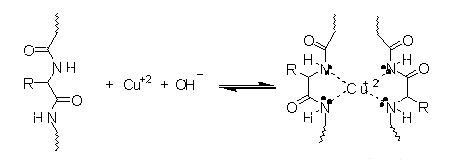
\includegraphics[width=\linewidth]{Biuret}
		\caption{Reacci\'on de Biuret.}
		\label{sch: Biuret}
	\end{scheme}

	Respecto a la prueba con ninhidrina, tanto para el h\'igado de pollo, e h\'igado de res, los resultados se contradicen entre ellos. Si bien ambas pruebas son generales, para las prote\'inas se debe tener en cuenta, que en el caso de la ninhidrina, la reacci\'on ocurre \'unicamente con el residuo terminal de un polip\'eptido, espec\'ificamente con el grupo amino libre. La reacci\'on se muestra en el \autoref{sch: ninhidrina}, y procede de la siguiente manera: la ninhidrina oxida y desamina el amino\'acido, formando 2-amino-1,3-indandiona, la cual posteriormente reacciona con una nueva mol\'ecula de ninhidrina, dando lugar a la formaci\'on del crom\'oforo violeta de Rheumann's. Sin embargo, por ejemplo para el caso del cerebro de res, es posible que la reacci\'on haya tenido lugar inicialmente con prolina, puesto que a partir de este amino\'acido se obtiene un compuesto anaranjado.
	
	Una posible explicaci\'on al por qu\'e los resultados de la ninhidrina contradicen los de Biuret, se encuentra relacionada con la concentraci\'on de los crom\'oforos, dado que la prueba de Biuret puede reaccionar potencialmente con todos los enlaces pept\'idicos de la muestra, mientras que la ninhidrina \'unicamente reacciona una vez con cada polip\'eptido.
	\begin{scheme}[h]
		\centering
		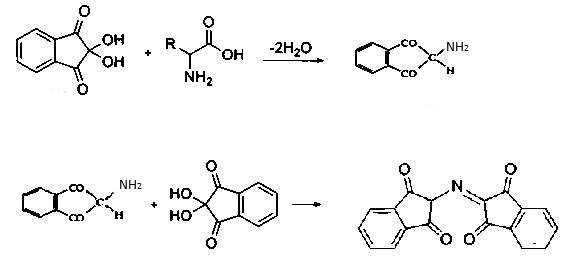
\includegraphics[width=\linewidth]{ninhydrin}
		\caption{Reacci\'on de los amino\'acidos con la ninhidrina.}
		\label{sch: ninhidrina}
	\end{scheme}

	\newpage

\section{Conclusiones}
	Fue posible determinar la presencia de carbohidratos, l\'ipidos y prote\'inas por duplicado para h\'igados de pollo y res, coraz\'on de pollo y cerebro de res. En el caso de los carbohidratos, en general la prueba de Lugol fue negativa en todos los casos, salvo por una muestra de coraz\'on de pollo, mientras que Molish siempre fue positivo sin importar el grupo ni el tejido confirmando la presencia de carbohidratos. La prueba de Benedict fue positiva para el h\'igado de res de manera consistente, sin embargo, para el h\'igado de pollo se obtuvieron resultados contradictorios, de manera an\'aloga a la prueba de Salkowsky. Finalmente, en el caso de las prote\'inas, se pudo determinar la presencia de las mismas en los tejidos usando la prueba de Biuret, la cual dio positiva en todos los casos, mientras que la reacci\'on con ninhidrina en el caso del h\'igado de pollo tuvo resultados contradictorios. Para terminar, se argumenta que no es posible una comparaci\'on entre tejidos, si los resultados para un mismo tejido, en una prueba cualitativa da lugar a distintas conclusiones, raz\'on por la cual, no se discute al respecto.
	
%----------------------------------------------------------------------------------------
%	REFERENCE LIST
%----------------------------------------------------------------------------------------
\phantomsection
\bibliography{informe}
\bibliographystyle{unsrt}

%----------------------------------------------------------------------------------------
%\newpage
%\onecolumn
%\section{Informaci\'on suplementaria}\label{sec: complementaria}
\end{document}